% \cleardoublepage

\newrefsection

\chapter{外文翻译: 在线带测试多处理器调度问题的随机算法}

论文标题:Randomized algorithms for fully online multiprocessor scheduling with testing

作者:Mingyang Gong等

\sectionnonum{摘要}

我们贡献了第一个随机化算法,该算法是任意多个确定性算法在完全在线多处理器调度与测试问题中的集成。
当只有两个机器时,我们展示了通过两个组件算法,其期望竞争比已经严格小于已证明的最佳确定性竞争比下界。
这种算法结果在文献中极为罕见。多处理器调度是最早得到大量研究的组合优化问题之一。
最近,多个研究小组研究了其测试变体,在该变体中,
每个作业 \( J_j \) 具有一个处理时间的上界 \( u_j \) 和一个长度为 \( t_j \) 的测试操作;
可以选择执行作业 \( J_j \) 的最大处理时间 \( u_j \),或者选择对 \( J_j \) 进行测试,
测试时间为 \( t_j \),以获得确切的处理时间 \( p_j \),然后立即执行该作业的 \( p_j \) 时间。
我们的目标问题是完全在线多处理器调度与测试问题,其中作业依次到达,
因此需要在作业到达时做出测试决策以及分配指定的机器。
我们首先利用 Yao 原理证明了至少三台机器情况下和仅两台机器情况下随机算法的期望竞争比下界分别为 1.6682 和 1.6522,
并提出了一个期望竞争比为 \( (\sqrt{\varphi' + 3} + 1)(\approx 3.1490) \)-竞争的随机算法,
该算法是通过一个非均匀概率分布集成了任意多个确定性算法,
其中 \( \varphi' = \frac{\sqrt{5}+1}{2} \) 是黄金比例。当只有两台机器时,
我们展示了基于两个确定性算法的随机化算法已经期望地 \( \frac{3\varphi + 3\sqrt{13 - 7\varphi}}{4}(\approx2.1839)\)-竞争,
同时证明了任何确定性算法的竞争比下界为 2.2117。\\
\textbf{关键词:} 调度问题;多处理器;带测试调度;完工时间;随机算法

\section{介绍}

我们在本文中研究完全在线的多处理器调度与测试问题~\cite{durr2018scheduling,durr2020adversarial,albers2021explorable,albers2021scheduling},
并从随机化算法的角度进行研究。多处理器调度~\cite{garey1979computers}是最早的已知 NP 难组合优化问题之一,在过去几十年中得到了广泛研究。多处理器调度的一个实例 \( I \) 包含一组 \( n \) 个作业 \( J = \{J_1, J_2, \dots, J_n\} \),每个作业都要在一组 \( m \) 台并行的相同机器 \( M = \{M_1, M_2, \dots, M_m\} \) 上非抢占地执行,目标是最小化最大完工时间 \( C_{\text{max}} \),即最大作业完成时间。与经典设置不同的是,在调度与测试中,每个作业 \( J_j \) 都有一个处理时间上界 \( u_j \),并且有一个长度为 \( t_j \) 的测试操作,但其处理时间 \( p_j \) 直到作业被测试后才会揭示。作业 \( J_j \) 可以在其中一台机器上执行 \( u_j \) 时间,或者选择先进行测试,测试时间为 \( t_j \),然后立即执行 \( p_j \) 时间。若所有作业都在时间零到达,则多处理器调度与测试是一个半在线问题,表示为 \( P | t_j, 0 \leq p_j \leq u_j | C_{\text{max}} \)。本文研究的是完全在线问题,其中作业按顺序到达,在作业到达时需要做出测试决策,并且指定测试和/或执行的机器,表示为 \( P | \text{online}, t_j, 0 \leq p_j \leq u_j | C_{\text{max}} \)。显然,半在线是完全在线的特例,在这两种情况下,调度器都应该利用已知的作业信息,在作业到达时决定是否进行测试,以便最好地平衡由于未知处理时间所消耗的总时间。

给定一个多项式时间的确定性算法,针对半在线或完全在线问题,令 \( C(I) \) 为该算法在实例 \( I \) 上产生的最大完工时间,而 \( C^*(I) \) 为最优离线调度的最大完工时间。算法的性能通过竞争比来衡量,定义为 \( \sup_I \{ C(I) / C^*(I) \} \),其中 \( I \) 遍历所有问题实例,算法称为 \( \sup_I \{ C(I) / C^*(I) \} \)-竞争的。切换到随机化算法时,我们相应地收集其在实例 \( I \) 上的期望最大完工时间 \( E[C(I)] \),该随机化算法称为 \( \sup_I \{ E[C(I)] / C^*(I) \} \)-竞争的。对于在线问题,随机化算法有时可以更好地处理不确定性,从而导致比最好的确定性算法更低的期望竞争比。我们为 \( P | \text{online}, t_j, 0 \leq p_j \leq u_j | C_{\text{max}} \) 提出了这样的一个随机化算法,并且进一步证明,当只有两台机器时,其期望竞争比严格小于任何确定性算法已证明的竞争比下界。

我们提醒读者,在我们的问题中,作业处理是非抢占的。
在文献中,研究人员还考虑了抢占式作业处理~\cite{durr2018scheduling,durr2020adversarial,albers2021explorable,albers2021scheduling},
其中任何测试或执行操作都可以被中断并稍后恢复,或者考虑了更为受限的测试抢占式变体~\cite{albers2021scheduling},在该变体中,已测试作业的测试和执行操作是非抢占的,但执行操作不必立即跟随测试操作,且不一定发生在同一台机器上。此外,我们的目标是最小化最大完工时间 \( C_{\text{max}} \),即最小最大目标;而另一个重要目标是最小化总作业完成时间,或者最小和目标,这也是受到了许多研究的关注~\cite{durr2018scheduling,durr2020adversarial,albers2021scheduling}。

\subsection{关于全在线问题的现有研究}

现有的针对完全在线问题 \( P | \text{online}, t_j, 0 \leq p_j \leq u_j | C_{\text{max}} \) 的近似算法,无论是确定性算法还是随机化算法,都不多。
我们首先区分一个特殊的情况,其中所有的测试操作时间均为单位时间,即对于每个作业 \( J_j \),有 \( t_j = 1 \),我们称之为均匀测试情况~\cite{durr2018scheduling,durr2020adversarial,albers2021scheduling},
表示为 \( P | \text{online}, t_j = 1, 0 \leq p_j \leq u_j | C_{\text{max}} \)。
注意,在一般的测试情况下,测试时间可以是任何非负值。
当只有一台机器时,机器上的作业处理顺序与最大完工时间无关。
这表明完全在线问题和半在线问题是相同的。第一组结果是关于半在线均匀测试问题 \( P_1 | t_j = 1, 0 \leq p_j \leq u_j | C_{\text{max}} \),
由 D¨urr 等人~\cite{durr2018scheduling,durr2020adversarial}提出。
他们提出,当 \( u_j \geq \varphi = \frac{\sqrt{5} + 1}{2} \) 时测试作业 \( J_j \),或者以概率 \( f(u_j) = \max \left( 0, \frac{u_j(u_j - 1)}{u_j(u_j - 1) + 1} \right) \) 测试它,
从而得到了一个确定性的 \( \varphi \)-竞争算法和一个期望的 4/3 竞争算法。
令 \( r_j = \frac{u_j}{t_j} \);Albers 和 Eckl~\cite{albers2021explorable}将上述两种算法扩展到一般测试情况下 \( P_1 | t_j, 0 \leq p_j \leq u_j | C_{\text{max}} \),
即当 \( r_j \geq \varphi \) 时测试作业 \( J_j \),或者以概率 \( f(r_j) \) 测试它,
分别达到了相同的竞争比和期望竞争比。作者们~\cite{durr2018scheduling,durr2020adversarial,albers2021explorable}证明了这两种算法是最优的,即 \( \varphi \) 是任何确定性算法的竞争比下界,
而 4/3 是任何随机化算法的期望竞争比下界,这一结果由 Yao 原理~\cite{yao1977probabilistic}得出。 

当至少有两台机器时,完全在线问题比半在线问题更为一般。Albers 和 Eckl~\cite{albers2021scheduling}提出了在列表调度规则~\cite{graham1966bounds}中测试作业 \( J_j \),即当 \( r_j \geq \varphi \) 时,按照该规则将每个作业分配到最空闲的机器上进行处理(可能是测试后执行)。他们证明了这样的算法是 \( \varphi(2 - \frac{1}{m}) \)-竞争的,且该分析是紧的,其中 \( m \) 是机器的数量。他们还证明了,即使在均匀测试情况下 \( P | \text{online}, t_j = 1, 0 \leq p_j \leq u_j | C_{\text{max}} \) 中,任何确定性算法的竞争比下界为 2~\cite{albers2021scheduling},并且对于两台机器的一般测试情况 \( P_2 | \text{online}, t_j, 0 \leq p_j \leq u_j | C_{\text{max}} \),即当只有两台机器时,其下界为 2.0953,这一结果也稍微更好~\cite{albers2021scheduling}。

\subsection{我们的成果}

对于完全在线和半在线的多处理器调度与测试问题,目标是最小化最大完工时间,我们已经看到,现有的随机化算法仅为单机器情况下的最优期望 \(\frac43\) 竞争算法~\cite{durr2018scheduling,durr2020adversarial,albers2021explorable}。
它们的期望竞争比严格小于任何确定性算法竞争比下界 \( \varphi \)。对于经典的在线多处理器调度问题,只有当 \( 2 \leq m \leq 5 \) 时,
Bartal 等人~\cite{bartal1992new} 和 Seiden~\cite{seiden2000online} 提出的算法的期望竞争比严格小于任何确定性算法的竞争比下界;
Albers~\cite{albers2002randomized} 提出的算法期望竞争比 1.916 也严格小于确定性下界 1.919,
但条件是只使用了三种离线最大完工时间下界。

在本文中,我们始终假设完全在线问题 \( P | \text{online}, t_j, 0 \leq p_j \leq u_j | C_{\text{max}} \) 中至少有两台机器。我们提出了一个几乎随机化的算法,它是任意多个组件确定性算法的集成,每个算法以一定的概率运行,并证明其期望竞争比最多为
\(
\sqrt{\left(1 - \frac{1}{m}\right)^2 \varphi^2 + 2\left(1 - \frac{1}{m}\right) + 1},
\)
其中 \( m \) 是机器的数量。这个期望竞争比随着 \( m \) 的增大而严格递增,严格小于 Albers 和 Eckl~\cite{albers2021scheduling}提出的最佳已知确定性算法的竞争比 \( \varphi(2 - \frac{1}{m}) \),并且当 \( m \) 趋于无穷大时,它逼近 \( (\sqrt{\varphi + 3} + 1) \approx 3.1490 \)。据我们所知,文献中的几乎随机化算法大多数是其组件确定性算法的均匀分布,而我们的算法则是第一个非均匀分布的任意多个组件算法。

当只有两台机器时,即对于 \( P_2 | \text{online}, t_j, 0 \leq p_j \leq u_j | C_{\text{max}} \),我们展示了在随机化算法中采用两个组件确定性算法导致的期望竞争比为
\(\dfrac{3\varphi + 3\sqrt{13 - 7\varphi}}{4} \approx 2.1839。\)

对于这个两台机器的情况,Albers 和 Eckl~\cite{albers2021scheduling} 证明了任何确定性算法的竞争比下界为 2.0953。
我们将其改进为 2.2117,从而证明我们的随机化算法在期望竞争比方面优于任何确定性算法。

\begin{figure}[t]
    \centering
    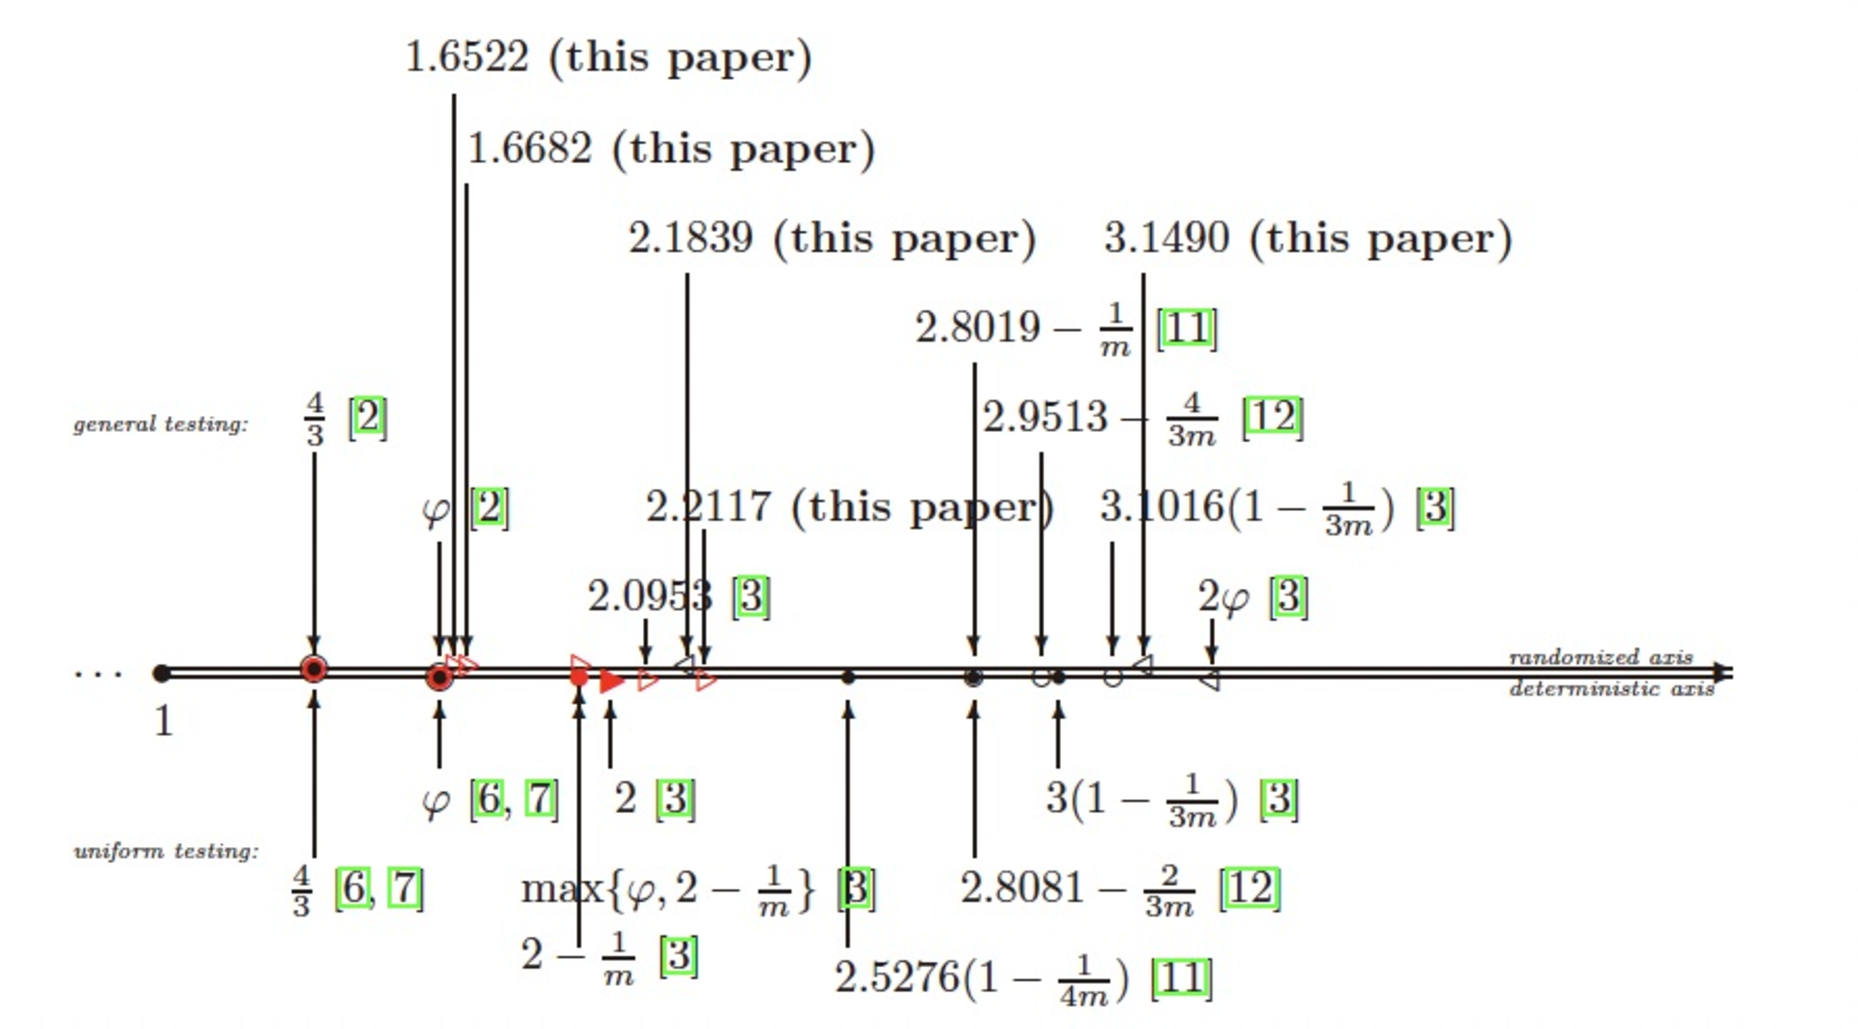
\includegraphics[width=.9\textwidth]{paper-results.pdf}
    \caption{现有的确定性和随机化算法在完全在线和半在线多处理器调度与测试问题中的竞争比。
    在横轴上,红色符号表示下界;三角形(\( \triangleleft \) 和 \( \triangleright \) 表示一般测试,否则表示均匀测试)
    表示完全在线问题的结果,而圆形(\(\circ\)表示一般测试,\(\cdot\)表示均匀测试)表示半在线问题的结果。
    在两个横轴之间,底部的轴表示确定性算法,顶部的轴表示随机化算法;
    轴上方的结果是针对一般测试情况的,而轴下方的结果是针对均匀测试情况的。
    }.
    \label{fig:paper-results}
\end{figure}

关于不可近似性,我们证明了至少三台机器时,任何随机化算法的期望竞争比下界为 1.6682,而在仅有两台机器时,对于 \( P_2 | \text{online}, t_j, 0 \leq p_j \leq u_j | C_{\text{max}} \),期望竞争比的下界为 1.6522,这两个下界都是使用稍微修改过的 Yao 原理~\cite{yao1977probabilistic} 得出的。
这两个下界在三台和两台机器情况下严格优于 Albers 和 Eckl~\cite{albers2021scheduling} 提出的下界 \( 2 - \frac{1}{m} \)。我们的所有结果总结如图~\ref{fig:paper-results}所示。

本文其余部分的组织结构如下:第 2 节介绍一些基本的符号和定义;接下来,在第 3 节中,我们证明了至少三台机器时完全在线问题 \( P | t_j, 0 \leq p_j \leq u_j | C_{\text{max}} \) 的期望竞争比下界 1.6682 和仅两台机器时的下界 1.6522;第 4 节包含了该问题的随机化算法及其性能分析、两台机器情况下稍微修改的随机化算法及其性能分析,以及对于 \( P_2 | \text{online}, t_j, 0 \leq p_j \leq u_j | C_{\text{max}} \) 的任何确定性算法的竞争比下界 2.2117;最后,第 5 节对论文进行了总结。

\section{预备内容}

我们研究完全在线的多处理器调度与测试问题,
以最小化最大完工时间,记作
\( P | \text{online}, t_j, 0 \leq p_j \leq u_j | C_{\text{max}} \),
其中作业依次到达。
我们的目标是设计期望竞争比优于现有最先进的确定性算法的随机化算法,
或者更进一步,优于已证明的最佳确定性竞争比下界。
所有作业都在时间零到达的特殊情况称为半在线问题,
记作 \( P | t_j , 0 \leq p_j \leq u_j | C_{\text{max}} \)。
在适用的情况下,我们将证明半在线变体的下界。

多处理器调度与测试的一个实例 \( I \) 
包含一组作业集 \( J = \{J_1, J_2, \dots, J_n\} \),
每个作业都要在一组 \( m \) 台并行的相同机器 
\( M = \{M_1, M_2, \dots, M_m\} \) 上执行,
其中 \( n \) 和 \( m \geq 2 \) 是输入的一部分。
每个作业 \( J_j \) 都有一个已知的处理时间上界 \( u_j \) 
和一个长度为 \( t_j \) 的测试操作,
处理时间 \( p_j \) 在测试操作执行之前是未知的。
也就是说,调度器可以选择不测试作业 \( J_j \),而是执行它 \( u_j \) 时间,
或者选择测试它 \( t_j \) 时间后,在同一台机器上立即执行 \( p_j \) 时间。

确定性算法 \( A \) 对是否测试作业做出二元决策。
令 \( p_{A_j} \) 和 \( \rho_j \) 
分别表示作业 \( J_j \) 在算法 \( A \) 和最优离线调度中的总时间。
可以看到,当作业被测试时,\( p_{A_j} = t_j + p_j \),
否则 \( p_{A_j} = u_j \),
而 \( \rho_j = \min\{u_j, t_j + p_j\} \)。
令 \( C_j \) 表示作业 \( J_j \) 在算法 \( A \) 生成的调度中的完成时间。
问题的目标是最小化最大完工时间 \( C_{\text{max}} = \max_j C_j \)。
我们使用 \( C_A(I) \)(当实例 \( I \) 在上下文中明确时,
简称为 \( C_A \))和 \( C^*(I) \)
(或相应的 \( C^* \))分别表示算法 \( A \) 和最优离线调度在实例 \( I \) 上的最大完工时间。

切换到更一般的随机化算法 \( A \),
其在实例 \( I \) 上的期望最大完工时间表示为 \( E[C_A(I)] \)。

\begin{defi}
    \textbf{竞争比:}
    对于确定性算法 \( A \),
    竞争比是算法 \( A \) 生成的调度的最大完工时间与最优离线调度的最大完工时间之间的最坏情况比值,即
    \[
    \sup_I \left\{ \frac{C_A(I)}{C^*(I)} \right\}
    \]
    其中 \( I \) 遍历所有问题实例。
\end{defi}

对于更一般的随机化算法 \( A \),其期望竞争比为

\[
\sup_I \left\{ \frac{E[C_A(I)]}{C^*(I)} \right\}
\]

由于作业 \( J_j \) 的处理时间 \( p_j \) 可能达到 0 和 \( u_j \) 两个极端值,确定性算法通常会设置一个阈值函数 \( r_j = \frac{u_j}{t_j} \) 用于二元测试决策。直观上,随机化算法应该以概率 \( f(r_j) \) 测试作业 \( J_j \),并且该概率函数应该随着比率 \( r_j \) 的增大而增大,且当 \( r_j \leq 1 \) 时,\( f(r_j) = 0 \)。

实际上,D¨urr 等人 [6, 7] 和 Albers 与 Eckl [2] 在他们的最优期望 4/3 竞争随机化算法中使用了如下的概率函数:

\[
f(r) = 
\begin{cases}
0, & \text{如果 } r \leq 1, \\
\frac{r(r-1)}{r(r-1)+1}, & \text{如果 } r > 1.
\end{cases}
\]

他们分别应用于单机器问题 \( P_1 | \text{online}, t_j = 1, 0 \leq p_j \leq u_j | C_{\text{max}} \) 和 \( P_1 | \text{online}, t_j, 0 \leq p_j \leq u_j | C_{\text{max}} \)。遗憾的是,他们的成功不能轻易扩展到多机器情况,因为他们性能分析中使用的一个关键事实是,对于单台机器,期望最大完工时间等于所有作业期望处理时间的总和。我们在下面展示,对于多台机器,如果一个随机化算法使用式(1)中的概率函数来测试作业,那么当机器数量趋近于无穷大时,它的期望竞争比将是无界的。

\section{期望竞争下界}

\begin{thm}
    对于任何随机算法 \( A_r \) 和任何随机实例 \( I_r \),\( A_r \) 的期望竞争比满足
    \[
    \sup_{I \in I} \frac{E[C_{A_r}(I)]}{C^*(I)} \geq \inf_{A \in A} \frac{E[C_A(I_r)]}{E[C^*(I_r)]},
    \]
    其中 \( E[C_A(I_r)] \) 和 \( E[C^*(I_r)] \) 分别是确定性算法 \( A \) 在实例 \( I_r \) 上的期望目标值和最优期望目标值。
\end{thm}

对于半在线单机均匀测试问题 \( P1 | t_j = 1, 0 \leq p_j \leq u_j | C_{\max} \),以下随机实例展示了期望竞争比的紧致下界 \(\frac{4}{3}\)
\cite{durr2018scheduling}\cite{durr2020adversarial}\cite{albers2021explorable}。

\begin{exm}
    在这个 \( P1 | t_j = 1, 0 \leq p_j \leq u_j | C_{\max} \) 的随机实例中,
    只有一个任务 \( J_1 \),其参数为 \( u_1 = 2 \) 和 \( t_1 = 1 \),且 \( p_1 = 0 \) 或 \( 2 \) 的概率各为0.5。

    在任何确定性算法 \( A \) 中,\( J_1 \) 要么被测试,要么未被测试。
    如果 \( J_1 \) 未被测试,则 \( p^A_1 = u_1 = 2 \);否则 \( J_1 \) 被测试,因此 \( p^A_1 = t_1 + p_1 \),这可能是1或3,每种情况的概率各为0.5。
    由此得出期望总执行时间为 \( E[p^A_1] = 2 \),无论 \( J_1 \) 是否被测试。
    
    另一方面,最优离线执行时间是 \( \rho_1 = 1 \) 如果 \( p_1 = 0 \),
    或者 \( \rho_1 = 2 \) 如果 \( p_1 = 2 \);即,期望最优执行时间为 \( E[\rho_1] = 1.5 \)。
    根据定理1,\( \frac{E[p^A_1]}{E[\rho_1]} = \frac{4}{3} \) 是半在线单机均匀测试问题 \( P1 | t_j = 1, 0 \leq p_j \leq u_j | C_{\max} \) 的期望竞争比的下界。    
\end{exm}

当有多台机器时,以下确定性实例展示了期望竞争比的下界 \( 2 - \frac{1}{m} \) \cite{albers2021scheduling}。

\begin{exm}
    在这个 \( P | t_j = 1, 0 \leq p_j \leq u_j | C_{\max} \) 的确定性实例中,
    有 \( m \) 台机器和 \( m \) 个任务 \( J_1, J_2, \ldots, J_m \),
    每个任务的参数为 \( u_j = 2 \) 和 \( t_j = 1 \),且 \( p_j = 0 \) 或 \( 2 \) 的概率各为0.5。

    在任何确定性算法 \( A \) 中,每个任务 \( J_j \) 要么被测试,要么未被测试。
    如果 \( J_j \) 未被测试,则 \( p^A_j = u_j = 2 \);否则 \( J_j \) 被测试,因此 \( p^A_j = t_j + p_j \),这可能是1或3,每种情况的概率各为0.5。
    由此得出每个任务的期望执行时间为 \( E[p^A_j] = 2 \)。
    
    考虑最优离线调度。如果所有任务 \( J_j \) 都未被测试,则每个任务的实际处理时间为2,总完成时间为 \( 2m \)。
    如果所有任务都被测试,则每个任务的实际处理时间是1或3,每种情况的概率各为0.5,总完成时间为 \( m \times 1.5 = 1.5m \)。
    最优离线调度可以通过将任务分配到不同的机器上来实现最小的完成时间。
    最优离线完成时间为 \( \rho = \frac{2m}{m} = 2 \) 如果所有任务都未被测试,或者 \( \rho = \frac{1.5m}{m} = 1.5 \) 如果所有任务都被测试。
    因此,期望最优完成时间为 \( E[\rho] = 1.5 \)。
    
    根据定理1,对于多台机器的情况,\( \frac{E[C_A]}{E[\rho]} = \frac{2m}{1.5m} = \frac{4}{3} \) 是一个下界。
    然而,通过更精细的分析,可以得到更紧致的下界 \( 2 - \frac{1}{m} \)。
    
    因此,对于多台机器的情况,期望竞争比的下界为 \( 2 - \frac{1}{m} \)。
\end{exm}

\begin{exm}
    在这个 \( P | \text{online}, t_j, 0 \leq p_j \leq u_j | C_{\max} \) 的确定性实例 \( I \) 中,
    有 \( m \) 台机器和 \( m + 1 \) 个任务按顺序到达 \( \langle J_1, J_2, \ldots, J_{m+1} \rangle \),每个任务的参数为
    \[ u_j = 2, \quad t_j = 1, \quad \text{对于任何 } j = 1, 2, \ldots, m + 1. \]
    也就是说,这 \( m + 1 \) 个任务在到达时是不可区分的。
    对于一个确定性算法,对手将前两个未被测试的任务(如果存在)或序列中的最后两个任务的实际执行时间设置为0;
    其他 \( m - 1 \) 个任务的实际执行时间为2。
    
    例如,当 \( m = 4 \) 且算法不测试任何任务时,实际执行时间序列为 \( \langle 0, 0, 2, 2, 2 \rangle \);
    如果算法不测试 \( J_3, J_4 \) 和 \( J_5 \) 中的任何一个,则实际执行时间序列为 \( \langle 2, 2, 0, 0, 2 \rangle \);
    如果算法仅不测试 \( J_1 \),则实际执行时间序列为 \( \langle 0, 2, 2, 2, 0 \rangle \);
    如果算法测试所有五个任务,则实际执行时间序列为 \( \langle 2, 2, 2, 0, 0 \rangle \)。
\end{exm}

给定一个确定性算法 \( A \),记 \( C^A_{\min}(I) \) 为算法 \( A \) 在实例 \( I \) 上产生的调度中的最小机器负载。

\begin{lem}
    当 \( m \geq 3 \) 时,在实例3中的实例 \( I \) 上,对于任何确定性算法 \( A \),
    要么 \( C_A(I) \geq 4 \),要么 \( C_A(I) = 3 \) 且 \( C_{\min}(I) \geq 2 \)。
\end{lem}

\begin{proof}
    如果算法 \( A \) 不测试两个或更多任务,则每个任务的总处理时间至少为2。根据鸽巢原理,这会导致完成时间 \( C_A(I) \geq 4 \)。
    如果算法 \( A \) 测试了所有任务中的至多一个任务,则在前 \( m \) 个任务 \( \langle J_1, J_2, \ldots, J_m \rangle \) 中,
    除了一个例外任务外,每个任务的总处理时间为3。这个例外任务的总处理时间如果是被测试的则为1,未被测试的则为2。
    可以看到,当一台机器被分配了这些 \( m \) 个任务中的任意两个时,根据鸽巢原理,完成时间 \( C_A(I) \geq 4 \)。
    在另一种情况下,每台机器恰好被分配了一个这些 \( m \) 个任务中的任务,将最后一个任务 \( J_{m+1} \) 分配给任何一台机器会导致
    要么 \( C_A(I) \geq 4 \),要么 \( C_A(I) = 3 \) 且 \( C_{\min}(I) \geq 2 \)。
\end{proof}

\begin{lem}
    当 \( m = 2 \) 时,在实例3中的实例 \( I \) 上,对于任何确定性算法 \( A \),
    要么 \( C_A(I) \geq 5 \),要么 \( C_A(I) \geq 4 \) 且 \( C_{\min}(I) \geq 1 \),
    要么 \( C_A(I) \geq 3 \) 且 \( C_{\min}(I) \geq 2 \)。
\end{lem}

\begin{proof}
    设 \( I \) 是一个三任务实例。我们区分两种情况:算法 \( A \) 是否测试第一个任务 \( J_1 \)。
    \begin{enumerate}
        \item \( J_1 \) 被测试。在这种情况下,\( p_1 = 2 \),从而 \( p^A_1 = 3 \)。注意到 \( J_2 \) 和 \( J_3 \) 的总处理时间至少为1。这三个值 \(\{3, 1, 1\}\) 保证了其中一个完成时间场景。
        \item \( J_1 \) 未被测试。在这种情况下,\( p_1 = 0 \),从而 \( p^A_1 = 2 \)。注意到 \( J_2 \) 和 \( J_3 \) 的总处理时间至少为2。这三个值 \(\{2, 2, 2\}\) 也保证了其中一个完成时间场景。
    \end{enumerate}
    因此,无论哪种情况,都可以保证完成时间 \( C_A(I) \geq 4 \) 或 \( C_A(I) = 3 \) 且 \( C_{\min}(I) \geq 2 \)。

    如果 \( J_1 \) 未被测试,则 \( p^A_1 = 2 \)。
    注意到 \( J_2 \) 和 \( J_3 \) 中的一个任务的总处理时间至少为2(要么未被测试,要么被测试且实际执行时间为2),另一个任务的总处理时间至少为1。
    这三个值 \(\{2, 2, 1\}\) 保证了其中一个完成时间场景。
\end{proof}

\begin{thm}
    对于存在三台或更多机器的情况 \( P | \text{online}, t_j, 0 \leq p_j \leq u_j | C_{\max} \),
    任何随机算法的期望竞争比至少为 \( \frac{21}{2} - \sqrt{78} \approx 1.6682 \)。

\end{thm}

\begin{thm}
    对于问题 \( P2 | \text{online}, t_j, 0 \leq p_j \leq u_j | C_{\max} \),
    任何随机算法的期望竞争比至少为 \( \frac{21 + 4\sqrt{51}}{30} \approx 1.6522 \)。
\end{thm}

\section{随机算法}

在本节中,我们首先提出了一种针对至少两台机器存在的完全在线多处理器调度与测试问题 
\( P | \text{online}, t_j, 0 \leq p_j \leq u_j | C_{\max} \) 的随机算法,
并证明其期望竞争比为 \( (\sqrt{\varphi} + 3 + 1) \approx 3.1490 \)。
当只有两台机器时,我们稍微调整了算法中的参数,
从而得到了改进的期望竞争比 \( \frac{3\varphi + 3\sqrt{13 - 7\varphi}}{4} \approx 2.1839 \)。
最后,我们证明了对于两台机器的情况,任何确定性算法的竞争比的改进下界为2.2117,
这意味着我们的随机算法在期望竞争比方面优于任何确定性算法。

对于完全在线多处理器调度与测试问题 \( P | \text{online}, t_j, 0 \leq p_j \leq u_j | C_{\max} \),
Albers和Eckl\cite{albers2021explorable} 提出如果 \( r_j \geq \varphi \) 则对任务 \( J_j \) 进行测试,
在列表调度规则 \cite{graham1966bounds} 中将每个任务分配给负载最小的机器进行处理(可能先测试后执行)。
他们证明了这种确定性算法是紧致的 \( \varphi(2 - \frac{1}{m}) \)-竞争比,其中 \( m \) 是机器的数量。
我们将它作为我们的第一个组合算法 \( A_0 \),
并以概率 \( \alpha_0 = \alpha(m, \ell) \) 运行该算法,如公式 \ref{eq:alpha0} 所示,
其中 \( \ell \geq 1 \) 是由我们的随机算法选择的一个固定常数。

\begin{equation}
    \alpha_0 = \alpha(m,l)
    = \sqrt{\dfrac{(1-\frac 1m)(l+1)\varphi^2}{(1-\frac 1m)(l+1)\varphi^2+2l}},
    a_i = \beta(m,l) = \dfrac{1-\alpha(m,l)}{l}, i = 1,2,\dots,l.
    \label{eq:alpha0}
\end{equation}

以下 \( \alpha(m, \ell) \) 和 \( \beta(m, \ell) \) 分别简写为 \( \alpha \) 和 \( \beta \)。

可以看到,当 \( r_j \leq 1 \) 时,任务 \( J_j \) 不应该被测试,
这在算法 \( A_0 \) 中也是如此。
另一方面,当 \( r_j \) 很大时,即使 \( p_j \) 非常接近 \( u_j \),
测试也不会浪费太多时间,这也与算法 \( A_0 \) 的情况一致。
“做出错误测试决策的风险”发生在 \( r_j \) 接近 \( \varphi \) 时,
因为在这种情况下,如果 \( J_j \) 未被测试,则 \( p_j \) 可能非常接近0;
而如果被测试,则 \( p_j \) 可能非常接近 \( u_j \)。然而,从引理1的证明中我们也可以看到,即使对具有较大比率 \( r_j \) 的任务进行不测试的概率很小,也可能导致期望竞争比无界,特别是在机器数量 \( m \) 趋于无穷大时。

因此,在其他每个组合算法 \( A_i \)(\( i = 1, 2, \ldots, \ell \))中,
我们设置一个阈值 \( y_i(m, \ell) > \varphi \) 如公式 \ref{eq:ratiolimit} 所示,
使得比率 \( r_j \geq y_i(m, \ell) \) 的任务 \( J_j \) 在 \( A_i \) 中被测试;
然后我们设置另一个阈值 \( x_i(m, \ell) = 1 + \frac{1}{y_i(m, \ell)} \),
使得比率 \( r_j \leq x_i(m, \ell) \) 的任务 \( J_j \) 在 \( A_i \) 中不被测试。

\begin{equation}
    y_i(m,l) = \dfrac{\varphi(\alpha+i\beta)}{\alpha},
    x_i(m,l) = 1 + \dfrac 1{y_i(m,l)},
    i = 0,1,\dots,l.
    \label{eq:ratiolimit}
\end{equation}

类似地,下面我们将 \( y_i(m, \ell) \) 和 \( x_i(m, \ell) \) 简化为 \( y_i \) 和 \( x_i \),分别表示。
当 \( r_j \in (x_i, y_i) \) 时,我们在 \( A_i \) 中反转测试决策,
即如果 \( r_j \leq \varphi \) 则测试 \( J_j \),如果 \( r_j > \varphi \) 则不测试 \( J_j \)。
我们的随机算法,记作GCL,以概率 \( \alpha_i \) 选择运行 \( A_i \),其中 \( i = 0, 1, \ldots, \ell \)。

从公式 \ref{eq:alpha0} 和 \ref{eq:ratiolimit} 可以看出,\( \alpha, \beta > 0 \),并且

\begin{equation}
    1 < x_\ell < \ldots < x_1 < x_0
    = \varphi = y_0 < y_1 < \ldots < y_\ell = \frac{\varphi}{\alpha}.
\end{equation}

算法GCL的简要描述如图2所示。

\begin{Thmbox}
    \begin{description}
        \item[输入:] \( m \) 台机器,以及按顺序到达的 \( n \) 个任务 \( \langle J_1, J_2, \ldots, J_n \rangle \);
        \item[输出:] 一个调度方案,其中每个任务被测试或不被测试,并指定处理该任务的机器。
        \item[步骤:]
        \begin{enumerate}
          \item 选择 \( \ell \),并根据公式 \ref{eq:alpha0} 和 \ref{eq:ratiolimit} 设置参数 \( \alpha_i, y_i \) 和 \( x_i \),对于 \( i = 0, 1, \ldots, \ell \);
          \item 组成算法 \( A_i \),\( i = 0, 1, \ldots, \ell \): 对于每个任务 \( J_j \),
            \begin{enumerate}
              \item 如果 \( r_j \leq x_i \) 或 \( \varphi < r_j \leq y_i \),则将 \( J_j \) 未测试地分配到负载最小的机器上进行处理;
              \item 否则,将 \( J_j \) 分配到负载最小的机器上进行测试和处理。
            \end{enumerate}
          \item 以概率 \( \alpha_i \) 选择运行 \( A_i \),对于 \( i = 0, 1, \ldots, \ell \)。
        \end{enumerate}
      \end{description}
\end{Thmbox}

\begin{lem}
\[
    \frac{1-\alpha}{x_i} < \frac{\alpha}{\varphi},
    (l-i)\beta(y_{i+1}-1) < \frac{\alpha}{\varphi},
    \forall i=0,1,\dots,\ell-1.
\]
\end{lem}

\begin{lem}
在算法 \( A_i \) 中,\( p_j^{A_i}\leq y_i\rho_j, \forall J_j, i=0,1,\dots,\ell \)。
\end{lem}

\begin{lem}
在算法 GCL 中,$E[p_j^A]\leq x_l\rho_j, \forall J_j$。
\end{lem}

\begin{thm}
    对于问题 \( P | \text{online}, t_j, 0 \leq p_j \leq u_j | C_{\max} \),
    若设置 \( \alpha(m, \ell) \) 和 \( \beta(m, \ell) \) 如公式 \ref{eq:alpha0} 所示,
    并且对于每一个 \( i = 0, 1, \ldots, \ell \) 
    设置 \( y_i(m, \ell) \) 和 \( x_i(m, \ell) \) 如公式 \ref{eq:ratiolimit} 所示,
    其中 \( m \geq 2 \) 是机器的数量,\( \ell \geq 1 \) 是一个固定的常数,
    则算法GCL的期望竞争比最多为
    \[
        \sqrt{(1 - \frac{1}{m})^2 (1 + \frac{1}{\ell})^2 \varphi^2 + 2(1 - \frac{1}{m})(1 + \frac{1}{\ell})} + 1 - (1 - \frac{1}{m}) \frac{\varphi}{\ell}
    \]
\end{thm}

通过选择一个足够大的 \( \ell \),算法GCL的期望竞争比接近
\( \sqrt{(1 - \frac{1}{m})^2 \varphi^2 + 2(1 - \frac{1}{m})} + 1 \)
该值随着 \( m \) 的增加而增加,并且当 \( m \) 趋于无穷大时,接近 \( \sqrt{\varphi + 3} + 1 \approx 3.1490 \)。
相应地,可以验证 \( \alpha, y_\ell \) 和 \( x_\ell \) 分别接近
\( \frac{\sqrt{\varphi} + 1}{\sqrt{\varphi} + 3} \approx 0.7529, \quad \sqrt{\varphi} + 3 \approx 2.1490, \quad 1 + \frac{1}{\sqrt{\varphi} + 3} \approx 1.4653. \)

在算法GCL中,我们可以将任务的测试概率 \( f(r) \) 作为其比率 \( r \) 的函数来确定。
例如,如果 \( r \geq y_\ell \),则 \( f(r) = 1 \);
如果 \( r \leq x_\ell \),则 \( f(r) = 0 \)。
对于一个固定的常数 \( \ell \),可以看到这种概率函数 \( f(r) \) 是阶梯状且递增的。
当 \( \ell \) 趋于无穷大时,这种概率函数的极限(仍然记作 \( f(r) \))是有趣的。
首先,注意到 \( \alpha(m, \ell) \) 接近 \( \alpha(m) = \sqrt{\frac{(1 - \frac{1}{m}) \varphi^2}{(1 - \frac{1}{m}) \varphi^2 + 2}} \),
\( y_\ell(m, \ell) \) 和 \( x_\ell(m, \ell) \) 分别接近 \( y(m) = \frac{\varphi}{\alpha(m)} \) 和 \( x(m) = 1 + \frac{1}{y(m)} \)。
然后,根据公式 \ref{eq:ratiolimit},我们有
\[
f(r) =
\begin{cases}
0, & \text{当 } r \leq x(m), \\
1 - \frac{\alpha(m)}{\varphi (r-1)}, & \text{当 } x(m) < r \leq \varphi, \\
\frac{\alpha(m) r}{\varphi}, & \text{当 } \varphi < r \leq y(m), \\
1, & \text{当 } r > y(m),
\end{cases}
\]
该函数是递增的,并且除了在 \( \varphi \) 处不连续外,在其他地方都是连续的。

当只有两台机器时,即 \( m = 2 \),通过选择一个足够大的 \( \ell \),
算法GCL对于问题 \( P2 | \text{online}, t_j, 0 \leq p_j \leq u_j | C_{\max} \) 
已经是期望 \( \frac{1}{2} \sqrt{\varphi + 5} + 1 \approx 2.2863 \)-竞争比。
注意,在算法内部,选择算法 \( A_0 \) 的概率接近 \( \alpha(2) = \frac{\varphi}{\sqrt{\varphi + 5}} \approx 0.6290 \)。

接下来我们展示,通过选择另一个运行 \( A_0 \) 的概率,
基于两个组成算法的修订后的GCL算法对于问题 \( P2 | \text{online}, t_j, 0 \leq p_j \leq u_j | C_{\max} \) 是
期望 \( \frac{3\varphi + 3\sqrt{13 - 7\varphi}}{4} \approx 2.1839 \)-竞争比。
进一步地,这个期望竞争比的界是紧的。

我们注意到,对于问题 \( P | \text{online}, t_j, 0 \leq p_j \leq u_j | C_{\max} \),
我们的GCL算法的期望竞争比优于已知的最佳确定性竞争比 \( \varphi(2 - \frac{1}{m}) \),
但远高于确定性竞争比的下界2 \cite{albers2021scheduling}。它更远离定理3中的1.6522、定理2中的1.6682
以及在两台、三台和 \( m \geq 4 \) 台机器存在的情况下期望竞争比的下界 \( 2 - \frac{1}{m} \) \cite{albers2021scheduling}。

回顾一下,除了对均匀测试情况 \( P | \text{online}, t_j = 1, 0 \leq p_j \leq u_j | C_{\max} \) 的确定性竞争比下界2之外,
Albers和Eckl \cite{albers2021scheduling} 还展示了两台机器一般测试情况 \( P2 | \text{online}, t_j, 0 \leq p_j \leq u_j | C_{\max} \) 的稍好一些的下界2.0953。我们在下一个定理中将该下界从2.0953改进到2.2117。因此,对于 \( P2 | \text{online}, t_j, 0 \leq p_j \leq u_j | C_{\max} \),
GCL的期望竞争比不仅优于半在线变体 \( P2 | t_j, 0 \leq p_j \leq u_j | C_{\max} \) 的已知最佳确定性竞争比2.3019,
而且优于完全在线问题的确定性竞争比下界2.2117。

\begin{thm}
    对于问题 \( P2 | \text{online}, t_j, 0 \leq p_j \leq u_j | C_{\max} \),
    任何确定性算法的竞争比大于2.2117。
\end{thm}

\begin{proof}

使用对抗性论证来构造一个三任务实例,任务顺序为 \( \langle J_1, J_2, J3 \rangle \)。
考虑一个确定性算法 \( A \)。

第一个任务 \( J_1 \) 的参数为 \( u_1 = \varphi \) 和 \( t_1 = 1 \)。
如果 \( A \) 测试 \( J_1 \),则对手设置 \( p_1 = \varphi \)。
因此 \( p^A_1 = \varphi + 1 \) 且 \( \rho_1 = \varphi \)。
如果 \( J_1 \) 未测试,则对手设置 \( p_1 = 0 \),
从而 \( p^A_1 = \varphi \) 且 \( \rho_1 = 1 \)。
无论哪种情况,都有 \( \frac{p^A_1}{\rho_1} = \varphi \),
因此我们假设 \( p^A_1 = \varphi \) 且 \( \rho_1 = 1 \)。
(如果 \( p^A_1 = \varphi + 1 \) 且 \( \rho_1 = \varphi \),
则下面与 \( J_2 \) 和 \( J_3 \) 相关的 \( u_j \) 和 \( t_j \) 值将乘以一个因子 \( \varphi \) 。)

对于任何即将到来的任务 \( J_j \)(即 \( j = 2, 3 \),
对手总是设置 \( p_j = u_j \) 如果 \( J_j \) 被算法测试,否则设置 \( p_j = 0 \)。

设 \( x_0 = \frac{3\varphi + 1 - \sqrt{11\varphi + 6}}{2} \approx 0.4878 \),这是二次方程 \( x^2 - (3\varphi + 1)x + \varphi^2 = 0 \) 的一个根。第二个任务 \( J_2 \) 的参数为 \( u_2 = \varphi - x_0 \) 和 \( t_2 = x_0 \)。我们区分两种情况:\( J_2 \) 是否被算法测试。

情况1: \( J_2 \) 被算法测试。
在这种情况下,\( p_2 = u_2 \) 且 \( p^A_2 = \varphi \) 且 \( \rho_2 = \varphi - x_0 \)。
如果 \( J_2 \) 被安排在与 \( J_1 \) 同一台机器上,
则第三个任务 \( J_3 \) 被取消(通过设置 \( u_j = t_j = 0 \)),导致 \( C_A = p^A_1 + p^A_2 = 2\varphi \)。
注意到 \( \rho_2 > 1 \) 且 \( C^* = \rho_2 = \varphi - x_0 \)。
因此竞争比为 \( \frac{2\varphi}{\varphi - x_0} \)。

下面假设 \( J_j \) 被分配到机器 \( M_j \) 上,
对于 \( j = 1, 2 \),每台机器的负载为 \( \varphi \)。
第三个任务 \( J_3 \) 的参数为 \( u_3 = y_0 \) 和 \( t_3 = \varphi + 1 - x_0 \),
其中 \( y_0 = \frac{1 - x_0 + \sqrt{(3\varphi - 5)x_0 + 15\varphi + 8}}{2} \approx 3.0933 \) 
是二次方程 \( y^2 - (1 - x_0)y - (\varphi + 1 - x_0)(2\varphi + 1 - x_0) = 0 \) 的一个根。

如果 \( J_3 \) 未被测试,则 \( p_3 = 0 \),从而 \( p^A_3 = y_0 \) 且 \( \rho_3 = \varphi + 1 - x_0 \),
导致 \( C_A = \varphi + y_0 \)。
在最优离线调度中,\( J_1 \) 和 \( J_2 \) 被安排在一台机器上,
而 \( J_3 \) 被安排在另一台机器上,导致最优离线完成时间为 \( C^* = \varphi + 1 - x_0 \)。
因此,竞争比为 \( \frac{C_A}{C^*} = \frac{y_0 + \varphi}{\varphi + 1 - x_0} \)。

如果 \( J_3 \) 被测试,则 \( p_3 = u_3 \),从而 \( p^A_3 = t_3 + u_3 = \varphi + 1 - x_0 + y_0 \) 且 \( \rho_3 = y_0 \),
导致 \( C_A = 2\varphi + 1 - x_0 + y_0 \)。
在最优离线调度中,\( J_1 \) 和 \( J_2 \) 被安排在一台机器上,
而 \( J_3 \) 被安排在另一台机器上,导致 \( C^* = y_0 \),
因此,竞争比为 \( \frac{C_A}{C^*} = \frac{2\varphi + 1 - x_0 + y_0}{y_0} \)。

综上所述,在这种情况下,我们有
\[
\frac{C_A}{C^*} \geq \min \left\{ \frac{2\varphi}{\varphi - x_0}, 
\frac{y_0 + \varphi}{\varphi + 1 - x_0}, 
\frac{2\varphi + 1 - x_0 + y_0}{y_0} \right\}.
\]

由于 \( y_0 \) 是二次方程 \( y^2 - (1 - x_0)y - (\varphi + 1 - x_0)(2\varphi + 1 - x_0) = 0 \) 的一个根,我们有
\[
y_0(y_0 + \varphi) = (\varphi + 1 - x_0)(y_0 + 2\varphi + 1 - x_0),
\]
即上述最后两个量相等且大约为2.21172。第一个量约为2.8634。
因此,\(\frac{C_A}{C^*} > 2.2117\)。

情况2: \( J_2 \) 未被算法测试。
在这种情况下,\( p_2 = 0 \),从而 \( p^A_2 = \varphi - x_0 \) 且 \( \rho_2 = x_0 \)。
如果 \( J_2 \) 被安排在与 \( J_1 \) 同一台机器上,
则第三个任务 \( J_3 \) 被取消(通过设置 \( u_j = t_j = 0 \)),
导致 \( C_A = p^A_1 + p^A_2 = 2\varphi - x_0 \)。
注意到 \( \rho_2 = x_0 < 1 \) 且 \( C^* = 1 \)。
因此,竞争比为 \( \frac{C_A}{C^*} = 2\varphi - x_0 \)。

下面假设 \( J_j \) 被分配到机器 \( M_j \) 上,
对于 \( j = 1, 2 \),两台机器的负载分别为 \( \varphi \) 和 \( \varphi - x_0 \)。
第三个任务 \( J_3 \) 的参数为 \( u_3 = \frac{(1+\varphi)y_0}{2\varphi+1-x_0} \approx 2.1606 \) 和 \( t_3 = 1 + x_0 \),其中 \( y_0 \) 与情况1相同。

如果 \( J_3 \) 未被测试,则 \( p_3 = 0 \),
从而 \( p^A_3 = u_3 = \frac{(1+\varphi)y_0}{2\varphi+1-x_0} \) 且 \( \rho_3 = 1 + x_0 \),无论 \( J_3 \) 被分配到哪台机器上,
都有 \( C_A \geq \varphi - x_0 + \frac{(1+\varphi)y_0}{2\varphi+1-x_0} \)。
在最优离线调度中,\( J_1 \) 和 \( J_2 \) 被安排在一台机器上,而 \( J_3 \) 被安排在另一台机器上,
导致最优离线完成时间为 \( C^* = 1 + x_0 \)。因此,竞争比为
\[
\frac{C_A}{C^*} \geq \frac{\varphi - x_0 + \frac{(1+\varphi)y_0}{2\varphi+1-x_0}}{1 + x_0} = \frac{(\varphi - x_0)(2\varphi + 1 - x_0) + (1 + \varphi)y_0}{(1 + x_0)(2\varphi + 1 - x_0)}.
\]
由于 \( x_0 \) 是二次方程 \( x^2 - (3\varphi + 1)x + \varphi^2 = 0 \) 的一个根,我们有
\[
(\varphi - x_0)(2\varphi + 1 - x_0) = x_0^2 - (3\varphi + 1)x_0 + \varphi(1 + 2\varphi) = \varphi(1 + \varphi)
\]
和
\[
(1 + x_0)(2\varphi + 1 - x_0) = -x_0^2 + 2\varphi x_0 + 2\varphi + 1 = (\varphi + 1)(1 + \varphi - x_0).
\]
因此,\(\frac{C_A}{C^*} \geq \frac{y_0 + \varphi}{1 + \varphi - x_0}\)。

如果 \( J_3 \) 被测试,则 \( p_3 = u_3 \),
从而 \( p^A_3 = t_3 + u_3 = 1 + x_0 + \frac{(1+\varphi)y_0}{2\varphi+1-x_0} \) 且 \( \rho_3 = \frac{(1+\varphi)y_0}{2\varphi+1-x_0} \),无论 \( J_3 \) 被分配到哪台机器上,都有 \( C_A \geq 1 + \varphi + \frac{(1+\varphi)y_0}{2\varphi+1-x_0} \)。由于 \( \rho_3 > \rho_1 + \rho_2 \),在最优离线调度中,\( J_1 \) 和 \( J_2 \) 被安排在一台机器上,
而 \( J_3 \) 被安排在另一台机器上,导致 \( C^* = \rho_3 = \frac{(1+\varphi)y_0}{2\varphi+1-x_0} \),进而竞争比为
\[
\frac{C_A}{C^*} \geq \frac{1 + \varphi + \frac{(1+\varphi)y_0}{2\varphi+1-x_0}}{\frac{(1+\varphi)y_0}{2\varphi+1-x_0}} = \frac{y_0 + 2\varphi + 1 - x_0}{y_0}.
\]

综上所述,在这种情况下,我们有
\[
\frac{C_A}{C^*} \geq \min \left\{ 2\varphi - x_0, 
\frac{y_0 + \varphi}{1 + \varphi - x_0}, 
\frac{2\varphi + 1 - x_0 + y_0}{y_0} \right\}.
\]

与情况1相同,上述最后两个量相等且大约为2.21172。第一个量约为2.7482。因此,\(\frac{C_A}{C^*} > 2.2117\)。

以上两种情况证明了对于问题 \( P2 | \text{online}, t_j, 0 \leq p_j \leq u_j | C_{\max} \),
任何确定性算法的竞争比大于2.2117。

\end{proof}

\section{结论}

我们研究了完全在线多处理器调度与测试问题 \( P | \text{online}, t_j, 0 \leq p_j \leq u_j | C_{\max} \),
并提出了一种随机算法GCL,该算法是非均匀分布的任意多个确定性算法。
据我们所知,文献中的随机算法作为元算法大多是其组成确定性算法的均匀分布,
而我们的GCL偏向于其中一个组成算法;
此外,当有多个组成算法时,以前的随机算法通常需要记录所有解,
而我们的GCL不需要这样做,因为组成算法彼此独立。
我们证明了GCL的期望竞争比约为3.1490。
当只有两台机器时,即对于 \( P2 | \text{online}, t_j, 0 \leq p_j \leq u_j | C_{\max} \),
使用修订后的GCL算法中的两个组成算法可以得到期望竞争比为2.1839。

我们还证明了三个不可近似结果,包括在至少三台机器存在的情况下,任何随机算法的期望竞争比的下界为1.6682,
对于 \( P2 | \text{online}, t_j, 0 \leq p_j \leq u_j | C_{\max} \) 的任何随机算法的期望竞争比的下界为1.6522,
以及对于 \( P2 | \text{online}, t_j, 0 \leq p_j \leq u_j | C_{\max} \) 的任何确定性算法的竞争比的下界为2.2117。根据最后一个下界,我们得出结论,算法GCL在期望竞争比方面优于任何确定性算法。这种算法结果在文献中很少见。

算法GCL的期望竞争比远高于两台、三台和\( m \geq 4 \)台机器情况下的下界1.6522、1.6682和\( 2 - \frac{1}{m} \),
这表明未来的研究可以缩小这些差距,即使是在两台机器的情况下也是如此。
可以看到,算法GCL中的任务比率测试概率函数在 \(\varphi\) 处不连续,
这暗示可能存在一个更好的概率分布函数来选择组成算法。

\begingroup
    \linespreadsingle{} 
    \printbibliography[title={外文翻译参考文献}]
\endgroup
